\chapter{Transferencia de calor en flujo multif\'asico bidimensional}
\label{chap:modelo2D}

La simulaci\'on de flujos multif\'asicos isot\'ermicos con LB comenz\'o pr\'acticamente con el origen del m\'etodo, y el desarrollo continuo de modelos ha permitido aplicar esta t\'ecnica a un amplio abanico de problemas. Sin embargo, a pesar del \'exito de LB en este \'area, la simulaci\'on de la transferencia de calor contin\'ua como un t\'opico abierto y en pleno desarrollo.

En el presente cap\'itulo se introduce un nuevo modelo para simular la transferencia de calor en flujos multif\'asicos, basado en una \lbe{} que permite recuperar adecuadamente una ecuaci\'on de energ\'ia consistente termodin\'amicamente con la aproximaci\'on pseudopotencial. El nuevo modelo, desarrollado formalmente para una grilla D2Q9, es validado con un conjunto de experimentos num\'ericos con soluci\'on anal\'itica. Aspectos tradicionales de la propuesta, como consistencia e independencia de grilla, son analizados a partir de la simulaci\'on de generaci\'on de burbujas sobre una superficie horizontal calefaccionada. Los principales resultados de este an\'alisis se encuentran publicados en \cite{fogliatto_assessment_2021}.


\section{Transporte de calor en lattice Boltzmann}

En general, los modelos LB existentes que permiten simular transferencia de calor en flujos multif\'asicos pueden clasificarse en tres categor\'ias principales: modelos de velocidad m\'ultiple (\emph{multi-speed}), modelos h\'ibridos (\emph{hybrid}) y modelos con dos funciones de distribuci\'on (\emph{double-distribution}). En el primer caso, las propiedades macrosc\'opicas del fluido como densidad, velocidad y temperatura, se obtienen a partir de los momentos cero, primero y segundo respectivamente de una \'unica funci\'on de distribuci\'on \cite{succi_lattice_2018,alexander_lattice_1993}. A pesar de que estos modelos cuentan con un s\'olido fundamento te\'orico, su difusi\'on es limitada, ya que t\'ipicamente emplean un conjunto de velocidades mayor que el correspondiente modelo isot\'ermico. Adem\'as, suelen incorporar t\'erminos de mayor orden en la \edf{} y est\'an restringidos a la simulaci\'on de un fluido con n\'umero de Prandtl constante.

Estas limitaciones intr\'insecas de los modelos de velocidad m\'ultiple motivaron el desarrollo de otro tipo de modelos t\'ermicos, donde se introduce un acoplamiento expl\'icito entre un esquema isot\'ermico para las ecuaciones hidrodin\'amicas, y una t\'ecnica alternativa para el transporte de energ\'ia. Los modelos h\'ibridos \cite{dong_numerical_2012,li_lattice_2015}, por un lado, aprovechan la discretizaci\'on del dominio asociada a la ecuaci\'on hidrodin\'amica, y hacen uso de un esquema cl\'asico de diferencias finitas para encontrar la soluci\'on de la ecuaci\'on de energ\'ia correspondiente. Por otro lado, los modelos con dos funciones de distribuci\'on introducen una segunda \lbe{} para recuperar la ecuaci\'on macrosc\'opica deseada.

Los esquemas de doble \fdp{} heredan las principales ventajas de LB, como simplicidad del algoritmo y elevada eficiencia computacional. Sin embargo, tambi\'en presentan las limitaciones comunes derivadas de la representaci\'on de ecuaciones escalares de advecci\'on-difusi\'on \cite{huang_multiphase_2015, markus_simulation_2011, huang_modified_2014, li_improved_2017, huang_numerical_2011, li_effect_2014}. En este tipo de ecuaciones hay una \'unica cantidad conservada (por ejemplo temperatura o energ\'ia), de modo que se relajan las condiciones de isotrop\'ia y es posible, en teor\'ia, emplear distribuciones de equilibrio lineales (en la velocidad del fluido) o conjuntos de velocidades reducidos. Sin embargo, la expansi\'on de Chapman-Enskog de estos esquemas muestra que existen t\'erminos no deseados que se recuperan inevitablemente en las ecuaciones macrosc\'opicas \cite{kruger_lattice_2017, huang_modified_2014, huang_numerical_2011}, y en el caso de los modelos para flujo multif\'asico con transferencia de calor, estos t\'erminos producen fuentes de calor adicionales que dependen del potencial de interacci\'on o de derivadas temporales de la velocidad del fluido.

Un ejemplo t\'ipico de estas restricciones puede analizarse con el uso de una \lbe{} con operador de colisi\'on SRT destinada a recuperar una ecuaci\'on de advecci\'on-difusi\'on de un escalar pasivo $\phi$:
\begin{equation}
	\dfrac{\partial \phi}{\partial t} + \nabla \cdot (\phi \bm{u}) = \nabla \cdot (k \nabla \phi),
	\label{eq:adv_dif_phi}
\end{equation}
donde $k$ es una constante de difusi\'on. En este caso, si se utiliza un esquema cl\'asico de LB para una \fdp{} $g$, es decir:
\begin{equation}
	\begin{gathered}
		g_{\alpha}(\bm{x}+\bm{e}_{\alpha}\delta_t, t+\delta_t) - g_{\alpha}(\bm{x},t) = -\dfrac{1}{\tau} \left[ g_{\alpha}(\bm{x},t) - g^{eq}_{\alpha}(\bm{x},t) \right], \\[2mm]
		g_{\alpha}^{eq} = w_i \phi \left[ 1 + \dfrac{e_{i\alpha}u_{\alpha}}{c_s^2} + \dfrac{u_{\alpha}u_{\beta}(e_{i\alpha}e_{i\beta}-c_s^2\delta_{\alpha\beta})}{2c_s^4} \right], \\[2mm]
		\phi = \sum_{\alpha} g_{\alpha},
	\end{gathered}
\end{equation}
entonces puede demostrarse que la ecuaci\'on macrosc\'opica recuperada para $\phi$ satisface:
\begin{equation}
	\dfrac{\partial \phi}{\partial t} + \nabla \cdot (\phi \bm{u}) = \nabla \cdot \left\{ \delta_t(\tau - 0.5) \left[ \dfrac{\partial (\phi\bm{u})}{\partial t} + \nabla \cdot (\phi \bm{uu}) + c_s^2 \nabla \phi\right]\right\}.
	\label{eq:adv_dif_phi_rec}
\end{equation}

En este caso, el coeficiente de difusi\'on recuperado est\'a dado por $k=c_s^2 \delta_t(\tau-0.5)$. A diferencia de la \eq{eq:adv_dif_phi}, la \eq{eq:adv_dif_phi_rec} contiene un t\'ermino de desviaci\'on dado por $\nabla \cdot \{ \delta_t(\tau - 0.5) [ \partial_t (\phi\bm{u}) + \nabla \cdot (\phi \bm{uu}) ]\}$, que puede anularse completamente s\'olo en aquellos casos con perfiles de velocidad especiales, como $\bm{u}=const$, $\bm{u}=[u_x(y),0]$, $\bm{u}=[0,u_y(x)]$, etc. 

Ejemplos similares pueden encontrarse dentro de los modelos \pp{} \cite{li_effect_2014}. En ciertas aplicaciones se desea recuperar una ecuaci\'on macrosc\'opica de la forma:
\begin{equation}
	\dfrac{\partial (\rho c_v T)}{\partial t} + \nabla \cdot (\rho c_v T \bm{u}) = \nabla \cdot (\lambda \nabla T),
\end{equation}
donde $\lambda$ es la conductividad t\'ermica y $c_v$ el calor espec\'ifico a volumen constante. En este caso el esquema usual consiste en utilizar una \lbe{} \pp{} est\'andar para la funci\'on de distribuci\'on $f$, asociada a las ecuaciones hidrodin\'amicas, mientras que este esquema tambi\'en puede utilizarse para una segunda distribuci\'on $g$, con $g^{eq}_{\alpha} = c_v T f^{eq}_{\alpha}$ y $\sum g_{\alpha} = \rho c_v T$. Nuevamente, la expansi\'on de Chapman-Enskog demuestra que la ecuaci\'on macrosc\'opica recuperada resulta:
\begin{equation}
	\dfrac{\partial (\rho c_v T)}{\partial t} + \nabla \cdot (\rho c_v T \bm{u}) = \nabla \cdot \left(\lambda \nabla T + \dfrac{\lambda}{p}T\bm{F} \right),
	\label{eq:e_macro_F}
\end{equation}
es decir, aparece un t\'ermino no deseado asociado a la fuerza total de la ecuaci\'on de impulso. Si estos t\'erminos son identificados, como en este caso, entonces pueden ser compensados expl\'icitamente:
\begin{equation}
	g_{\alpha}(\bm{x}+\bm{e}_{\alpha}\delta_t, t+\delta_t) - g_{\alpha}(\bm{x},t) = -\dfrac{1}{\tau} \left[ g_{\alpha}(\bm{x},t) - g^{eq}_{\alpha}(\bm{x},t) \right] + \delta_t C_{\alpha}(\bm{x},t),
\end{equation}
donde $C_{\alpha}$ es un t\'ermino de correcci\'on:
\begin{equation}
	C_{\alpha} = \left( 1-\dfrac{1}{2\tau} \right)\omega_{\alpha}c_v T \dfrac{\bm{e}_{\alpha} \cdot \bm{F}}{c_s^2}.
\end{equation}

%\nomenclature[N]{$\lambda$}{Conductividad t\'ermica}
%\nomenclature[N]{$c_v$}{Calor espec\'ifico a volumen constante}

En definitiva, los modelos de doble \fdp{} resultan atractivos, ya que permiten conservar la elegancia y simpleza propia de lattice Boltzmann, mientras que aportan una mayor flexibilidad en el tipo de ecuaciones macrosc\'opicas que pueden recuperarse. Sin embargo, si se desea incrementar la aplicabilidad de estos modelos hacia problemas m\'as complejos, es necesario desarrollar un mecanismo natural para eliminar los t\'erminos no deseados en la ecuaci\'on macrosc\'opica recuperada. Por lo tanto, siguiendo este objetivo primario, en la secci\'on siguiente se introduce un modelo alternativo que permite remediar satisfactoriamente estas limitaciones.


\section{Ecuaci\'on de energ\'ia con operador MRT}
El modelo \pp{} de Li ha sido extensamente validado en la bibliograf\'ia, donde se ha demostrado que puede utilizarse exitosamente en la simulaci\'on de flujos multif\'asicos bidimensionales, con Re moderados y relaci\'on de densidades elevadas (hasta $\rho_l / \rho_g \sim 750$). Adicionalmente, los resultados de la simulaci\'on de un fluido vdW mostrados en el \chap{chap:isot} y en \cite{fogliatto_simulation_2019}, sugieren que el modelo es capaz de incorporar adecuadamente fuerzas externas sin afectar la correcci\'on sobre la inconsistencia termodin\'amica. El an\'alisis de convergencia en malla, que en este contexto se traduce en un incremento de unidades de grilla conservando par\'ametros adimensionales, muestra que es posible alcanzar una precisi\'on adecuada en la reproducci\'on de interfases. Sin embargo, si se desea expandir su uso hacia la simulaci\'on de flujos multif\'asicos con transferencia de calor y cambio de fase, entonces es necesario proveer un nuevo esquema para cuantificar adecuadamente el transporte de energ\'ia.

Dentro del contexto de modelos \pps{}, donde se consideran fluidos cuya presi\'on termodin\'amica se encuentra gobernada por una \eos{}, la ecuaci\'on de energ\'ia macrosc\'opica debe seguir una forma particular. Tomando como base un balance local de entrop\'ia, y despreciando efectos de disipaci\'on viscosa, M\'arkus y H\'azi derivaron una ecuaci\'on macrosc\'opica para la energ\'ia, representada por medio de la temperatura \cite{markus_simulation_2011}:
\begin{equation}
	\dfrac{\partial T}{\partial t} + \bm{u} \cdot \nabla T = \dfrac{1}{\rho c_v} \nabla \cdot(\lambda \nabla T) - \dfrac{T}{\rho c_v} \left( \dfrac{\partial p_{EOS}}{\partial T} \right)_{\rho} \nabla \cdot \bm{u}.
	\label{eq:markus_orig}
\end{equation}
La \eq{eq:markus_orig} consiste en una ecuaci\'on de advecci\'on-difusi\'on para $T$, con un t\'ermino de fuente asociado al trabajo de compresi\'on. En las secciones siguientes se considerar\'a que la difusividad t\'ermica $\chi = \lambda/(\rho c_v)$ y el calor espec\'ifico $c_v$ son constantes en cada fase, de modo que la \eq{eq:markus_orig} puede reescribirse como:
\begin{equation}
	\dfrac{\partial T}{\partial t} + \nabla \cdot (\bm{u} T) = \chi \nabla^2 T  + \dfrac{\chi}{\rho} \nabla T \cdot \nabla \rho + T \left[ 1 - \dfrac{1}{\rho c_v} \left( \dfrac{\partial p_{EOS}}{\partial T} \right)_{\rho} \right] \nabla \cdot \bm{u}.
	\label{eq:markus}
\end{equation}
%\nomenclature[N]{$\chi$}{Difusividad t\'ermica}

Esta aproximaci\'on, si bien implica una p\'erdida de generalidad, facilita el desarrollo del esquema LB. Por otro lado, como se describe en las secciones siguientes,  la forma original de la ecuaci\'on puede recuperarse usando t\'erminos de fuente adecuados. 

El desarrollo de un modelo puede originarse en el an\'alisis sobre la simulaci\'on de ecuaciones de advecci\'on-difus\'on llevado a cabo por Huang y colaboradores \cite{huang_modified_2014, huang_numerical_2011, huang_lattice_2015}: la recuperaci\'on de una ecuaci\'on escalar usando una \lbe{} con operador de colisi\'on MRT permite combinar aquellos momentos responsables de los t\'erminos no deseados. Si esta interacci\'on se lleva a cabo de forma inteligente, entonces es posible lograr la supresi\'on de componentes espec\'ificos dentro de las escalas de expansi\'on analizadas. Por otro lado, como se desea recuperar un t\'ermino de fuente, \'este debe incorporarse al esquema sin la adici\'on de derivadas convectivas de dicha fuente \cite{cheng_introducing_2008}, lo que fuerza a la incorporaci\'on de un t\'ermino de fuente impl\'icito. Combinando estas ideas, una \lbe{} adecuada para recuperar la \eq{eq:markus} resulta:

\begin{equation}
	\begin{aligned}
		\tilde{\bm{g}}(\bm{x} + \bm{e} \delta_t, t+\delta_t) &=
		\tilde{\bm{g}}(\bm{x}, t) - (\bm{M}^{-1}Q\bm{M}) \left[ \tilde{\bm{g}}(\bm{x}, t) - \tilde{\bm{g}}^{eq}(\bm{x}, t) \right] \\
		&  + \dfrac{\delta_t}{2} \hat{\bm{\Gamma}}(\bm{x},t) + \hat{\bm{\Gamma}}(\bm{x} +\bm{e}\delta_t,t + \delta_t),
	\end{aligned}
	\label{eq:g_tilde_2d}	
\end{equation}

\begin{equation}
	\sum_{\alpha} \tilde{g}_{\alpha} = T.
\end{equation}

Siguiendo la notaci\'on usada previamente para las \lbe{} con operador MRT, la componente $\alpha$-\'esima del miembro izquierdo de la \eq{eq:g_tilde_2d} corresponde  a $\tilde{g}_{\alpha}(\bm{x}+\bm{e}_{\alpha}\delta_t, t+\delta_t)$, y $\bm{M}$ a la matriz de transformaci\'on al espacio de momentos (\eq{eq:MRT_M_D2Q9}).  En este caso, $\bm{Q}$ corresponde a una matriz de coeficientes relajaci\'on y $\hat{\bm{\Gamma}} = \bm{M}^{-1}\bm{\Gamma}$ a un t\'ermino de fuente en el espacio de poblaciones. Como la \eq{eq:g_tilde_2d} contiene una fuente impl\'icita, puede transformarse usando:
\begin{equation}
	g_{\alpha}(\bm{x},t) = \tilde{g}_{\alpha} (\bm{x},t) - \dfrac{\delta_t}{2} \hat{\Gamma}_{\alpha}(\bm{x},t),
	\label{eq:g_tilde_tranf_2d}
\end{equation}
de modo que el momento de orden cero resulta:
\begin{equation}
	\begin{aligned}
		T &= \sum_{\alpha} \tilde{g}_{\alpha} \\
		  &= \sum_{\alpha} g_{\alpha} + \dfrac{\delta_t}{2} \sum_{\alpha} \tilde{\Gamma}_{\alpha} \\
		  &= \sum_{\alpha} g_{\alpha} + \dfrac{\delta_t}{2} \Gamma_0.
	\end{aligned}
	\label{eq:T_macro_2d}
\end{equation}
En la \eq{eq:T_macro_2d} se utiliza que la primera fila de $\bm{M}$ corresponde a $\bm{M}_0 = (1, \cdots ,1)$, de forma que $T$ puede obtenerse usando la distribuci\'on $g$ y la primer componente de la fuente en el espacio de momentos. La \eq{eq:g_tilde_2d} puede reescribirse usando la \eq{eq:g_tilde_tranf_2d} como:
\begin{equation}
	\bm{g}(\bm{x} + \bm{e} \delta_t, t+\delta_t) = \bm{M}^{-1} \left[ \bm{n} - \bm{Q}(\bm{n} - \feq{n}) + \delta_t \left( \bm{I}-\dfrac{\bm{Q}}{2}\right) \bm{\Gamma}\right],
	\label{eq:g_model_2d}
\end{equation}
donde $\bm{n} = \bm{Mg}$ y se omiti\'o la dependencia $(\bm{x},t)$ por claridad. 

La determinaci\'on de la ecuaci\'on macrosc\'opica  recuperada puede hacerse mediante una expansi\'on de Chapman-Enskog, considerando las ideas expuestas en la \se{sec:chapman}. En primer lugar, es necesario reescribir el t\'ermino izquierdo de la \eq{eq:g_model_2d} empleando un desarrollo de Taylor para cada componente, es decir:
\begin{equation}
	g_{\alpha}(\bm{x}+\bm{e}_{\alpha}\delta_t,t+\delta_t) = \sum_{k=0}^{\infty} \dfrac{1}{k!}\delta_t^k D_{\alpha}^{k} \, g_{\alpha} \sim g_{\alpha} + \delta_t D_{\alpha} g_{\alpha} + \dfrac{1}{2}\delta_t^2 D_{\alpha}^2g_{\alpha},
	\label{eq:taylor_gral}
\end{equation}
donde $D_{\alpha} = \partial_t + \bm{e}_{\alpha} \cdot \nabla=\partial_t + e_{\alpha \beta} \partial_{\beta}$. Para escribir la \eq{eq:taylor_gral} en forma vectorial, es necesario definir las matrices diagonales $\bm{E}_{\beta} = diag(e_{0\beta} \cdots e_{q-1\beta})$ y $\bm{\nabla}_{\beta} = \partial_{\beta} \bm{I}$, de modo que la \eq{eq:taylor_gral} puede transformarse como:
\begin{equation}
	\bm{g}(\bm{x}+\bm{e}\delta_t. t+\delta_t) = \bm{g} 
	+ \delta_t\left( \dfrac{\partial}{\partial t} \bm{I} + \bm{E}_{\beta}\bm{\nabla}_{\beta} \right) \bm{g}
	+ \dfrac{\delta^2_t}{2} \left( \dfrac{\partial}{\partial t} \bm{I} + \bm{E}_{\beta}\bm{\nabla}_{\beta} \right)^2 \bm{g}.
	\label{eq:taylor_vec}
\end{equation}

Reemplazando la \eq{eq:taylor_vec} en la \eq{eq:g_model_2d} y multiplicando ambos miembros por $\bm{M}$, se obteniene una \lbe{} desarrollada en torno a $(\bm{x},t)$:
\begin{equation}
	\begin{aligned}
	\delta_t \bm{M}\left( \dfrac{\partial}{\partial t} \bm{I} + \bm{E}_{\beta}\bm{\nabla}_{\beta} \right) \bm{g} + \dfrac{\delta^2_t}{2} \bm{M}\left( \dfrac{\partial}{\partial t} \bm{I} + \bm{E}_{\beta}\bm{\nabla}_{\beta} \right)^2 \bm{g} 
	&= -\bm{Q}(\bm{n} - \feq{n}) \\
	& + \delta_t \left( \bm{I}-\dfrac{\bm{Q}}{2}\right) \bm{\Gamma}.
	\end{aligned}
	\label{eq:taylor_vec_2}
\end{equation}

S\'olo resta reescribir el miembro izquierdo de la \eq{eq:taylor_vec_2} para obtener una ecuaci\'on expresada completamente en el espacio de momentos. En particular, las derivadas de $\bm{g}$ pueden reescribirse como:
\begin{equation}
	\begin{aligned}
		\delta_t \bm{M}\left( \dfrac{\partial}{\partial t} \bm{I} + \bm{E}_{\beta}\bm{\nabla}_{\beta} \right) \bm{g} &= \delta_t \dfrac{\partial}{\partial t}\bm{IMg} + \delta_t ( \bm{M} \bm{E}_{\beta} \bm{M}^{-1} )( \bm{M} \bm{\nabla}_{\beta} \, \bm{g}) \\
		&= \delta_t \dfrac{\partial}{\partial t}\bm{In} + \delta_t \hat{\bm{E}}_{\beta} \bm{\nabla}_{\beta} \bm{n} \\
		&= \delta_t\left( \dfrac{\partial}{\partial t}\bm{I} + \hat{\bm{E}}_{\beta} \bm{\nabla}_{\beta} \right) \bm{n}
	\end{aligned}
	\label{eq:M_propag_1}
\end{equation}
y
\begin{equation}
	\begin{aligned}
		\dfrac{\delta^2_t}{2} \bm{M}\left( \dfrac{\partial}{\partial t} \bm{I} + \bm{E}_{\beta}\bm{\nabla}_{\beta} \right)^2 \bm{g} 
		&= \dfrac{\delta^2_t}{2} \left( \dfrac{\partial}{\partial t}\bm{I} + \hat{\bm{E}}_{\beta} \bm{\nabla}_{\beta} \right) \bm{M} \left( \dfrac{\partial}{\partial t}\bm{I} + \bm{E}_{\beta} \bm{\nabla}_{\beta} \right) \bm{g} \\
		&= \dfrac{\delta^2_t}{2} \left( \dfrac{\partial}{\partial t}\bm{I} + \hat{\bm{E}}_{\beta} \bm{\nabla}_{\beta} \right) \left( \dfrac{\partial}{\partial t}\bm{I} + \hat{\bm{E}}_{\beta} \bm{\nabla}_{\beta} \right) \bm{Mg} \\
		&= \dfrac{\delta^2_t}{2} \left( \dfrac{\partial}{\partial t}\bm{I} + \hat{\bm{E}}_{\beta} \bm{\nabla}_{\beta} \right)^2 \bm{n},
	\end{aligned}
	\label{eq:M_propag_2}
\end{equation}
donde se definen las matrices $\hat{\bm{E}}_{\beta} = \bm{M} \bm{E}_{\beta} \bm{M}^{-1}$. En una grilla D2Q9, donde $\beta=x$ o $\beta=y$, estas matrices resultan:
\begin{equation}
	\hat{\bm{E}}_{x}=
	\begin{bmatrix}
	0 & 0 & 0 & 1 & 0 & 0 & 0 & 0 & 0 \\
	0 & 0 & 0 & 1 & 1 & 0 & 0 & 0 & 0 \\
	0 & 0 & 0 & 0 & 1 & 0 & 0 & 0 & 0 \\
	2/3 & 5/3 & 0 & 0 & 0 & 0 & 0 & 1/2 & 0 \\
	0 & 1/3 & 1/3 & 0 & 0 & 0 & 0 & -1 & 0 \\
	0 & 0 & 0 & 0 & 0 & 0 & 0 & 0 & 1 \\
	0 & 0 & 0 & 0 & 0 & 0 & 0 & 0 & 1 \\
	0 & 0 & 0 & 1/3 & -1/3 & 0 & 0 & 0 & 0 \\
	0 & 0 & 0 & 0 & 0 & 2/3 & 1/3 & 0 & 0 \\
	\end{bmatrix},
\end{equation} 

\begin{equation}
	\hat{\bm{E}}_{y}=
	\begin{bmatrix}
	0 & 0 & 0 & 0 & 0 & 1 & 0 & 0 & 0 \\
	0 & 0 & 0 & 0 & 0 & 1 & 1 & 0 & 0 \\
	0 & 0 & 0 & 0 & 0 & 0 & 1 & 0 & 0 \\
	0 & 0 & 0 & 0 & 0 & 0 & 0 & 0 & 1 \\
	0 & 0 & 0 & 0 & 0 & 0 & 0 & 0 & 1 \\
	2/3 & 5/3 & 0 & 0 & 0 & 0 & 0 & 1/2 & 0 \\
	0 & 1/3 & 1/3 & 0 & 0 & 0 & 0 & 1 & 0 \\
	0 & 0 & 0 & 0 & 0 & -1/3 & 1/3 & 0 & 0 \\
	0 & 0 & 0 & 2/3 & 1/3 & 0 & 0 & 0 & 0 \\
	\end{bmatrix}.
\end{equation} 

Finalmente, reemplazando las \eqs{eq:M_propag_1}{eq:M_propag_2} en la \eq{eq:taylor_vec_2}, puede obtenerse una ecuaci\'on expresada completamente en el espacio de momentos, y definida en $(\bm{x},t)$:
\begin{equation}
	\dcm \bm{n} + \dfrac{\delta_t}{2} \dcm^2 \bm{n} = -\dfrac{1}{\delta_t}\bm{Q}(\bm{n} - \feq{n}) + \delta_t \left( \bm{I}-\dfrac{\bm{Q}}{2}\right) \bm{\Gamma}.
	\label{eq:model_2d_momento}
\end{equation}

Una vez que se tiene el desarrollo en serie de Taylor de una \lbe{} en torno a $(\bm{x},t)$, es necesario aplicar la expansi\'on de las \fdp{} y operadores diferenciales utilizando un par\'ametro de expansi\'on $\varepsilon$:

\begin{subequations}
	\begin{equation}
		\bm{n} = \bc{n}{0} + \varepsilon \bc{n}{1} + \varepsilon^2 \bc{n}{2} + \cdots = \sum_{k=0}^{\infty} \varepsilon^k \bc{n}{k},
		\label{eq:n_chapman}
	\end{equation}
	\begin{equation}
		\dfrac{\partial}{\partial t} = \varepsilon \dfrac{\partial}{\partial t_1} + 	\varepsilon^2 \dfrac{\partial}{\partial t_2},
	\end{equation}
	\begin{equation}
		\dfrac{\partial}{\partial x_{\beta}} = \varepsilon \dfrac{\partial}{\partial x_{\beta_1}},
	\end{equation}
	\begin{equation}
		\bm{\Gamma} = \varepsilon \bc{\Gamma}{1}.
		\label{eq:gamma_chapman}
	\end{equation}
	\label{eq:escalas_che}
\end{subequations}

Las expansiones determinadas por las \eqto{eq:n_chapman}{eq:gamma_chapman} pueden incorporarse a la \eq{eq:model_2d_momento}, y si se desprecian los t\'erminos de orden superior a $\varepsilon^2$ se obtiene:
\begin{equation}
	\begin{aligned}
		\varepsilon \dcmuno \bc{n}{0} + \varepsilon^2 \dcmuno \bc{n}{1} + \varepsilon^2 \dfrac{\partial}{\partial t_2} \bm{I} \bc{n}{0} \\
		+ \varepsilon^2 \dfrac{\delta_t}{2} \dcmuno^2 \bc{n}{0} = -\dfrac{1}{\delta_t} \bm{Q} \left( \bc{n}{0} + \varepsilon \bc{n}{1} + \varepsilon^2 \bc{n}{2} - \feq{n} +  \right) \\
		+ \varepsilon \left( \bm{I}-\dfrac{\bm{Q}}{2}\right) \bc{\Gamma}{1}
	\end{aligned}
	\label{eq:modelo_2d_escalas}
\end{equation}

De esta manera, con las variables y operadores diferenciales reemplazados por las expansiones correspondientes, puede generarse un conjunto de ecuaciones (una para cada potencia de $\varepsilon$) a partir de la separaci\'on de la \eq{eq:modelo_2d_escalas}:

\begin{subequations}
	\begin{align}
		\varepsilon^0: \, & \bc{n}{0} = \feq{n}\\
		\varepsilon^1: \, & \dcmuno \bc{n}{0} = -\dfrac{1}{\delta_t} \bm{Q} \bc{n}{1} + \left( \bm{I}-\dfrac{\bm{Q}}{2}\right) \bc{\Gamma}{1} \label{eq:eps_1_0} \\	
		\varepsilon^2: \, & { \dcmuno \bc{n}{1} + \dfrac{\partial \bc{n}{0}}{\partial t_2}  + \dfrac{\delta_t}{2} \dcmuno^2 \bc{n}{0}  = -\dfrac{1}{\delta_t} \bm{Q} \bc{n}{2}} \label{eq:eps_2_0}
	\end{align}
\end{subequations}


Usando la \eq{eq:eps_1_0} para reescribir el t\'ermino cuadr\'atico de la \eq{eq:eps_2_0}, y reagrupando t\'erminos, puede escribirse el conjunto de ecuaciones correspondientes a cada escala de expansi\'on:
\begin{subequations}
	\begin{align}
		\varepsilon^0: \, & \bc{n}{0} = \feq{n} \label{eq:eps_0}\\
		\varepsilon^1: \, & \dcmuno \bc{n}{0} - \bc{\Gamma}{1} = -\dfrac{1}{\delta_t} \bm{Q} \left( \bc{n}{1} + \dfrac{\delta_t}{2} \bc{\Gamma}{1} \right)  \label{eq:eps_1}\\
		\varepsilon^2: \, & \dcmuno \left( \bm{I}-\dfrac{\bm{Q}}{2}\right) \left( \bc{n}{1} + \dfrac{\delta_t}{2} \bc{\Gamma}{1} \right) + \dfrac{\partial \bc{n}{0}}{\partial t_2}  =  -\dfrac{1}{\delta_t} \bm{Q} \bc{n}{2} \label{eq:eps_2}
	\end{align}
\end{subequations}

El reordenamiento de t\'erminos utilizado en la construcci\'on de las \eqto{eq:eps_0}{eq:eps_2} permite visualizar expl\'icitamente el v\'inculo resultante entre cada escala: el t\'ermino de fuente de cada escala (en este caso, el miembro derecho), corresponde a la variable transportada en la escala de orden inmediatamente superior.

Hasta este punto, el an\'alisis sirve para hacer expl\'icito el proceso de separaci\'on de escalas determinado por la expansi\'on de Chapman-Enskog, desarrollado con el objetivo de encontrar la ecuaci\'on recuperada a partir de la \eq{eq:g_model_2d}. Sin embargo, para finalizar el proceso es necesario definir a la \edf{} y la matriz de coeficientes de relajaci\'on, dado que todav\'ia no se hizo uso de una forma expl\'icita de las mismas. Siguiendo con las ideas expuestas en los trabajos de Huang y sus colaboradores, la recuperaci\'on de una ecuaci\'on macrosc\'opica escalar reduce las restricciones de isotrop\'ia sobre el conjunto de velocidades. Adem\'as, como no es necesario recuperar t\'erminos del tipo $\nabla \cdot(\rho \bm{uu})$, es factible construir una distribuci\'on de equilibrio que s\'olo contenga t\'erminos hasta primer orden en la velocidad del fluido. Como esta distribuci\'on es utilizada dentro de un esquema de colisi\'on MRT resulta m\'as sencillo si se construye directamente en el espacio de momentos:
\begin{equation}
	\feq{n} = T(1, \alpha_1, \alpha_2, \alpha_3 u_x, \alpha_4 u_x, \alpha_5 u_y, \alpha_6 u_y, 0, 0 )^T.
\end{equation}
En este caso, las constantes $\{ \alpha_i \}$ constituyen un conjunto de par\'ametros libres que ser\'an empleados para determinar propiedades de la ecuaci\'on recuperada. Esta nueva distribuci\'on de equilibrio preserva el orden de los momentos de grilla establecidos por $\bm{M}$, pero a diferencia de la \eq{eq:feq_li}, no se consideran los t\'erminos cuadr\'aticos de $\bm{u}$.

Por otro lado, la \'unica restricci\'on impuesta hasta el momento sobre los coeficientes de la matriz $\bm{Q}$ es que sean constantes. En los operadores MRT tradicionales esta matriz es diagonal, y cada coeficiente se asocia a la relajaci\'on individual del momento correspondiente. Sin embargo, en las \eqs{eq:eps_1}{eq:eps_2} es posible ver que si $\bm{Q}$ tambi\'en contiene elementos no nulos fuera de la diagonal principal, se logra que las ecuaciones para cada componente incorporen tambi\'en otros momentos dentro de la misma escala de $\varepsilon$. De esta forma, con una elecci\'on de coeficientes adecuada se podr\'ian cancelar t\'erminos macrosc\'opicos no deseados. Para este caso, se propone que $\bm{Q}$ sea de la forma:

\begin{equation}
	\bm{Q}=
	\begin{bmatrix}
	q_0 & 0 & 0 & 0 & 0 & 0 & 0 & 0 & 0 \\
	0 & q_1 & 0 & 0 & 0 & 0 & 0 & 0 & 0 \\
	0 & 0 & q_2 & 0 & 0 & 0 & 0 & 0 & 0 \\
	0 & 0 & 0 & q_3 & q_{34} & 0 & 0 & 0 & 0 \\
	0 & 0 & 0 & 0 & q_4 & 0 & 0 & 0 & 0 \\
	0 & 0 & 0 & 0 & 0 & q_5 & q_{56} & 0 & 0 \\
	0 & 0 & 0 & 0 & 0 & 0 & q_6 & 0 & 0 \\
	0 & 0 & 0 & 0 & 0 & 0 & 0 & q_7 & 0 \\
	0 & 0 & 0 & 0 & 0 & 0 & 0 & 0 & q_8 \\
	\end{bmatrix},
\end{equation} 
\FloatBarrier
donde los coeficientes $q_{34}$ y $q_{56}$ ser\'an definidos convenientemente.  

Con la definici\'on expl\'icita de $\feq{n}$ y $\bm{Q}$ es posible completar el an\'alisis de expansi\'on multiescala. En particular es necesario evaluar, dentro de cada escala, aquellos componentes correspondientes a las cantidades conservadas. Como en este caso s\'olo se tiene $T$, se necesitan \'unicamente los primeros componentes (\'indice 0). Para la escala $\varepsilon$, de la \eq{eq:eps_1} se tiene:
\begin{equation}
	\dfrac{ \partial \nce{0}{0}}{\partial t_1}  +  \dfrac{ \partial \nce{3}{0}}{\partial x_1} + \dfrac{ \partial \nce{5}{0}}{\partial y_1} - \Gamma_0^{(1)}= -\dfrac{q_0}{\delta_t} \left( \nce{0}{1} + \dfrac{\delta_t}{2} \Gamma_0^{(1)} \right),
\end{equation}

\begin{equation}
	\dfrac{ \partial T}{\partial t_1}  +  \dfrac{ \partial (\alpha_3 T u_x)}{\partial x_1} + \dfrac{ \partial (\alpha_5 T u_y)}{\partial y_1} = -\dfrac{q_0}{\delta_t} \left( \nce{0}{1} + \dfrac{\delta_t}{2} \Gamma_0^{(1)} \right) + \Gamma_0^{(1)}.
	\label{eq:T_eps_1}
\end{equation}

Como
\begin{equation}
	T = \sum_{\alpha} g_{\alpha} + \dfrac{\delta_t}{2} \Gamma_0 = n_0 + \dfrac{\delta_t}{2} \Gamma_0
\end{equation}
y por las \eqs{eq:n_chapman}{eq:eps_0} se cumple:
\begin{equation}
	n_0 = \nce{0}{0} + \varepsilon \nce{0}{1} + \varepsilon^2 \nce{0}{2} + \cdots = n_0^{eq} + \varepsilon \nce{0}{1} + \varepsilon^2 \nce{0}{2} + \cdots,
\end{equation}
entonces dentro de cada escala se satisface:
\begin{equation}
	\begin{aligned}
		\varepsilon^0: && \nce{0}{0} = n_0^{eq} \\
		\varepsilon^1: && \nce{0}{1} + \dfrac{\delta_t}{2} \Gamma_0^{(1)} = 0\\
		\varepsilon^2: && \nce{0}{2} = 0 \\
		&\vdots& \\
		\varepsilon^k: && \nce{0}{k} = 0 \quad \forall \, k > 2.
	\end{aligned}
	\label{eq:ncero_che}
\end{equation}

Por lo tanto, si se usa $\alpha_3 = \alpha_5 = 1$, la \eq{eq:T_eps_1} finalmente se reduce a:
\begin{equation}
	\dfrac{\partial T}{\partial t_1} + \nabla_1 \cdot (T\bm{u}) = \Gamma_0^{(1)}.
	\label{eq:T_eps_1_macro}
\end{equation}

Por otro lado, para la escala $\varepsilon^2$ se necesita la primera componente de la \eq{eq:eps_2}:
\begin{equation}
	\begin{split}
	\dfrac{\partial \nce{0}{0}}{\partial t_2} + \dfrac{\partial}{\partial t_1}\left( 1-\dfrac{q_0}{2} \right) \left( \nce{0}{1} +\dfrac{\delta_t}{2} \Gamma_0^{(1)}\right) \\
	+ \dfrac{\partial}{\partial x_1}\left[ \left( 1-\dfrac{q_3}{2} \right) \left( \nce{3}{1} +\dfrac{\delta_t}{2} \Gamma_3^{(1)}\right) - \dfrac{q_{34}}{2} \left( \nce{4}{1} +\dfrac{\delta_t}{2} \Gamma_4^{(1)}\right) \right] \\
	+ \dfrac{\partial}{\partial y_1}\left[ \left( 1-\dfrac{q_5}{2} \right) \left( \nce{5}{1} +\dfrac{\delta_t}{2} \Gamma_5^{(1)}\right) - \dfrac{q_{56}}{2} \left( \nce{6}{1} +\dfrac{\delta_t}{2} \Gamma_6^{(1)}\right) \right] = -\dfrac{1}{\delta_t} q_0 \nce{0}{2}
	\end{split}.
	\label{eq:eps_2_comp_0}
\end{equation}

En la \eq{eq:eps_2_comp_0} aparecen diferentes componentes del t\'ermino de fuente $\bm{\Gamma}$. En esta etapa, se propone el uso de una fuente sencilla con una \'unica componente no nula, es decir:
\begin{equation}
	\bm{\Gamma} = (s,0,0,0,0,0,0,0,0)^T.	
\end{equation}

De esta manera, como $\Gamma = \varepsilon \Gamma^{(1)}$, entonces la \'unica componente no nula es $\Gamma_0^{(1)}$. Usando adem\'as la \eq{eq:ncero_che}, puede reescribirse la \eq{eq:eps_2_comp_0} como:
\begin{equation}
	\dfrac{\partial T}{\partial t_2} + 
	\underbrace{\dfrac{\partial}{\partial x_1}\left[ \left( 1-\dfrac{q_3}{2} \right) \nce{3}{1} - \dfrac{q_{34}}{2} \nce{4}{1} \right]}_{I} 	+  \underbrace{ \dfrac{\partial}{\partial y_1}\left[ \left( 1-\dfrac{q_5}{2} \right) \nce{5}{1} - \dfrac{q_{56}}{2}  \nce{6}{1} \right]}_{II} = 0	.
	\label{eq:eps_2_reduced}
\end{equation}

Como se observa en la \eq{eq:eps_2_reduced}, son necesarias ecuaciones para $\nce{3}{1}$, $\nce{4}{1}$, $\nce{5}{1}$ y $\nce{6}{1}$, las cuales pueden obtenerse de la \eq{eq:eps_2}. Por ejemplo, para $\nce{3}{1}$ se tiene:
\begin{equation}
	\dfrac{\partial \nce{3}{0}}{\partial t_1} + \dfrac{2}{3}\dfrac{\partial \nce{0}{0}}{\partial x_1} + \dfrac{1}{6}\dfrac{\partial \nce{1}{0}}{\partial x_1} - \Gamma_3^{(1)} = -\dfrac{q_3}{\delta_t} \left( \nce{3}{1} +\dfrac{\delta_t}{2} \Gamma_3^{(1)}\right) - \dfrac{q_{34}}{\delta_t} \left( \nce{4}{1} +\dfrac{\delta_t}{2} \Gamma_4^{(1)}\right),
\end{equation}
y reemplazando componentes:
\begin{equation}
	\dfrac{\partial (Tu_x)}{\partial t_1} + \dfrac{\partial}{\partial x_1} \left(\dfrac{4+\alpha_1}{6} T \right) = -\dfrac{q_3}{\delta_t} \nce{3}{1} - \dfrac{q_{34}}{\delta_t} \nce{4}{1}.
	\label{eq:n3_2d}
\end{equation}

Por otro lado, para $\nce{4}{1}$ se obtiene:
\begin{equation}
	\dfrac{\partial \nce{4}{0}}{\partial t_1} + \dfrac{1}{3}\dfrac{\partial \nce{1}{0}}{\partial x_1} + \dfrac{1}{1}\dfrac{\partial \nce{2}{0}}{\partial x_1}  + \dfrac{\partial \nce{8}{0}}{\partial y_1} - \dfrac{\partial \nce{7}{0}}{\partial x_1}	
	= -\dfrac{q_4}{\delta_t} \left( \nce{4}{1} +\dfrac{\delta_t}{2} \Gamma_4^{(1),}\right)
\end{equation}
\begin{equation}
	\dfrac{\partial (\alpha_4 Tu_x)}{\partial t_1} + \dfrac{\partial}{\partial x_1} \left(\dfrac{\alpha_1 + \alpha_2}{3} T \right) = -\dfrac{q_4}{\delta_t} \nce{4}{1}.
	\label{eq:n4_2d}
\end{equation}

Las ecuaciones \eqs{eq:n3_2d}{eq:n4_2d} pueden usarse para despejar $\nce{3}{1}$ y $\nce{4}{1}$, y poder as\'i reescribir el t\'ermino $I$ de la \eq{eq:eps_2_reduced}. Si se reemplazan dichas componentes, considerando $\alpha_4 = -1$, $I$ puede escribirse como:
\begin{equation}
\begin{aligned}
	I =& -\delta_t \left( \dfrac{1}{q_3} - \dfrac{1}{2}  + \dfrac{q_{34}}{q_3 q_4}  \right) \dfrac{\partial (Tu_x)}{\partial t_1} - \delta_t \left( \dfrac{1}{q_3} - \dfrac{1}{2} \right) \dfrac{\partial}{\partial x_1} \left(\dfrac{4+\alpha_1}{6} T \right) \\
	&+ \dfrac{q_{34}\delta_t}{q_3q_4}\dfrac{\partial}{\partial x_1} \left(\dfrac{\alpha_1+\alpha_2}{3} T \right).
	\label{eq:I_0}
\end{aligned}
\end{equation}


En la \eq{eq:I_0} puede apreciarse la utilidad de considerar una matriz $\bm{Q}$ con elementos no nulos fuera de la diagonal, ya que estos elementos pueden elegirse convenientemente para eliminar t\'erminos no deseados en las ecuaciones recuperadas. En particular, el t\'ermino con $\partial_{t_1}(Tu_x)$ puede cancelarse si se anula la combinaci\'on de factores de relajaci\'on que lo multiplican, es decir:
\begin{equation}
	q_{34} = q_4 \left( \dfrac{q_3}{2} - 1 \right).
\end{equation}

Con esta elecci\'on, la \eq{eq:I_0} finalmente puede reescribirse como:
\begin{equation}
	I = -\delta_t \left( \dfrac{1}{q_3} - \dfrac{1}{2} \right) \dfrac{\partial}{\partial x_1} \left(\dfrac{4+3\alpha_1 + 2\alpha_2}{6} T \right).
	\label{eq:I_1}
\end{equation}

Este resultado es fundamental para el desarrollo de modelos que busquen recuperar ecuaciones de advecci\'on-difusi\'on para variables escalares, ya que puede demostrarse formalmente que una elecci\'on adecuada de los coeficientes extra-diagonales de la matriz de relajaci\'on, lleva a la cancelaci\'on de aquellos t\'erminos no deseados en la ecuaci\'on macrosc\'opica. En este caso, con la definici\'on correcta de $q_{34}$ es posible eliminar $\partial_{t_1}(Tu_x)$ en las escalas de expansi\'on analizadas.

El mismo procedimiento puede realizarse para reescribir el término denotado como $II$ en la \eq{eq:eps_2_reduced}: despejando $\nce{5}{1}$ y $\nce{6}{1}$ de las componentes 5 y 6 de la \eq{eq:eps_2}, y usando $\alpha_6=-1$, $II$ puede reescribirse como:
\begin{equation}
\begin{aligned}
	II =& -\delta_t \left( \dfrac{1}{q_5} - \dfrac{1}{2}  + \dfrac{q_{56}}{q_5 q_6}  \right) \dfrac{\partial (Tu_y)}{\partial t_1} - \delta_t \left( \dfrac{1}{q_5} - \dfrac{1}{2} \right) \dfrac{\partial}{\partial y_1} \left(\dfrac{4+\alpha_1}{6} T \right) \\
	&+ \dfrac{q_{56}\delta_t}{q_5q_6}\dfrac{\partial}{\partial y_1} \left(\dfrac{\alpha_1+\alpha_2}{3} T \right).
	\label{eq:II_0}
\end{aligned}
\end{equation}
Por lo tanto, si 
\begin{equation}
	q_{56} = q_6 \left( \dfrac{q_5}{2} - 1 \right),
\end{equation}
entonces la \eq{eq:II_0} se reduce a:
\begin{equation}
	II = -\delta_t \left( \dfrac{1}{q_5} - \dfrac{1}{2} \right) \dfrac{\partial}{\partial y_1} \left(\dfrac{4+3\alpha_1 + 2\alpha_2}{6} T \right).
	\label{eq:II_1}
\end{equation}

Las \eqs{eq:I_1}{eq:II_1} pueden finalmente utilizarse para completar el an\'alisis en la escala $\varepsilon^2$:
\begin{equation}
	\begin{split}
	\dfrac{\partial T}{\partial t_2} -
	\dfrac{\partial}{\partial x_1}\left[ \delta_t \left( \dfrac{1}{q_3} - \dfrac{1}{2} \right) \dfrac{\partial}{\partial x_1} \left(\dfrac{4+3\alpha_1 + 2\alpha_2}{6} T \right) \right]	\\
	-  \dfrac{\partial}{\partial y_1}\left[ \delta_t \left( \dfrac{1}{q_5} - \dfrac{1}{2} \right) \dfrac{\partial}{\partial y_1} \left(\dfrac{4+3\alpha_1 + 2\alpha_2}{6} T \right) \right] = 0.
	\end{split}
	\label{eq:eps_2_clean}
\end{equation}

En particular, si adem\'as se impone $q_3=q_5=q_{\chi}$, entonces la \eq{eq:eps_2_clean} puede reescribirse como:

\begin{equation}
	\dfrac{\partial T}{\partial t_2} - \nabla_1 \cdot \left[ \delta_t \left( \dfrac{1}{q_{\chi}} - \dfrac{1}{2} \right) \, \nabla\left( \dfrac{4+3\alpha_1 + 2\alpha_2}{6} T \right) \right]  = 0.
	\label{eq:T_eps_2}
\end{equation}

Esta parte del an\'alisis de Chapman-Enskog implic\'o encontrar la descripci\'on del comportamiento de las variables macrosc\'opicas en las escalas de $\varepsilon$ propuestas, de modo que s\'olo resta volver a las escalas originales. Por lo tanto, multiplicando por $\varepsilon$ a la \eq{eq:T_eps_1_macro}, por $\varepsilon^2$ a la \eq{eq:T_eps_2} y sum\'andolas, se tiene:
\begin{equation}
	\varepsilon \dfrac{\partial T}{\partial t_1} + \varepsilon^2 \dfrac{\partial T}{\partial t_2} + \varepsilon \nabla_1 \cdot (T\bm{u}) - \varepsilon^2 \nabla_1 \cdot (\chi \nabla T) - \varepsilon \Gamma_0^{(1)} = 0,
\end{equation}
donde se define a la difusividad t\'ermica $\chi$ como:
\begin{equation}
	\chi = \delta_t \left( \dfrac{1}{q_{\chi}} - \dfrac{1}{2} \right) \left( \dfrac{4+3\alpha_1 + 2\alpha_2}{6} \right).
	\label{eq:modelo_2d_chi}
\end{equation}

Usando la expansi\'on de escalas dada por la \eq{eq:escalas_che}, la ecuaci\'on macrosc\'opica recuperada finalmente resulta:
\begin{equation}
	\dfrac{\partial T}{\partial t} + \nabla \cdot (T\bm{u}) = \nabla \cdot (\chi \nabla T) + s.
	\label{eq:T_2d}
\end{equation}

El procedimiento desarrollado para mostrar que la \eq{eq:g_model_2d} produce una temperatura macrosc\'opica que satisface la \eq{eq:T_2d}, resalta propiedades fundamentales de la propuesta. Por un lado, la construcci\'on \emph{ad-hoc} de una distribuci\'on de equilibrio directamente en el espacio de momentos, de una matriz de relajaci\'on con coeficientes no nulos fuera de la diagonal, y de un t\'ermino fuente definido directamente en el espacio de momentos, permite recuperar una ecuaci\'on de advecci\'on-difusi\'on para $T$ sin los t\'erminos no deseados caracter\'isticos de esquemas tradicionales. Por otro lado, la nueva distribuci\'on de equilibrio $\feq{n}$ contiene dos par\'ametros libres, $\alpha_1$ y $\alpha_2$, que permiten ajustar la difusividad t\'ermica recuperada sin necesidad de modificar el coeficiente de relajaci\'on $q_{\chi}$. Esta flexibilidad permite, en principio, mejorar los l\'imites de estabilidad del modelo.

La \eq{eq:T_2d} es similar a la ecuaci\'on objetivo de M\'arkus y H\'azi (\eq{eq:markus}), aunque el t\'ermino de fuente $s$ debe ser definido correctamente para incorporar expl\'icitamente las componentes faltantes. En definitiva, reuniendo las propuestas y suposiciones realizadas, es posible expresar lo siguiente a modo de s\'intesis del nuevo modelo \cite{fogliatto_assessment_2021}: la ecuaci\'on diferencial para $T$
\begin{equation}
	\dfrac{\partial T}{\partial t} + \nabla \cdot (\bm{u} T) = \chi \nabla^2 T  + \dfrac{\chi}{\rho} \nabla T \cdot \nabla \rho + T \left[ 1 - \dfrac{1}{\rho c_v} \left( \dfrac{\partial p_{EOS}}{\partial T} \right)_{\rho} \right] \nabla \cdot \bm{u}
\end{equation}
puede recuperarse usando una funci\'on de distribuci\'on $g$ que satisfaga la siguiente \lbe{} en el espacio de momentos:
\begin{subequations}
	\begin{equation}
		\bm{g}(\bm{x} + \bm{e} \delta_t, t+\delta_t) = \bm{M}^{-1} \left[ \bm{n} - \bm{Q}	(\bm{n} - \feq{n}) + \delta_t \left( \bm{I}-\dfrac{\bm{Q}}{2}\right) \bm{\Gamma}\right],		
	\end{equation}
	\begin{equation}
		\bm{n} = \bm{Mg}
	\end{equation}
	\begin{equation}
		T = \sum_{\alpha} g_{\alpha} + \dfrac{\delta_t}{2} \Gamma_0,		
	\end{equation}
	\begin{equation}
		\feq{n} = T(1, \alpha_1, \alpha_2, u_x, -u_x, u_y, -u_y, 0, 0 )^T,
	\end{equation}
	\begin{equation}
		\bm{\Gamma} = (s,0,0,0,0,0,0,0,0)^T,		
	\end{equation}
	\begin{equation}
		s = \dfrac{\chi}{\rho} \nabla T \cdot \nabla \rho + T \left[ 1 - \dfrac{1}{\rho c_v} \left( \dfrac{\partial p_{EOS}}{\partial T} \right)_{\rho} \right] \nabla \cdot \bm{u}
		\label{eq:model2D_hs}
	\end{equation}
	\begin{equation}
	 	\bm{Q}=
		\begin{bmatrix}
		q_0 & 0 & 0 & 0 & 0 & 0 & 0 & 0 & 0 \\
		0 & q_1 & 0 & 0 & 0 & 0 & 0 & 0 & 0 \\
		0 & 0 & q_2 & 0 & 0 & 0 & 0 & 0 & 0 \\
		0 & 0 & 0 & q_{\chi} & q_{34} & 0 & 0 & 0 & 0 \\
		0 & 0 & 0 & 0 & q_4 & 0 & 0 & 0 & 0 \\
		0 & 0 & 0 & 0 & 0 & q_{\chi} & q_{56} & 0 & 0 \\
		0 & 0 & 0 & 0 & 0 & 0 & q_6 & 0 & 0 \\
		0 & 0 & 0 & 0 & 0 & 0 & 0 & q_7 & 0 \\
		0 & 0 & 0 & 0 & 0 & 0 & 0 & 0 & q_8 \\
		\end{bmatrix},	
	\end{equation}
	\begin{equation}
		q_{34} = q_4 \left( \dfrac{q_{\chi}}{2} - 1 \right),
	\end{equation}
	\begin{equation}
		q_{56} = q_6 \left( \dfrac{q_{\chi}}{2} - 1 \right).
	\end{equation}
	\label{eq:modelo_2d_full}
\end{subequations}

Esta nueva \lbe{} puede acoplarse junto con la propuesta pseudopotencial de Li para poder simular flujos multif\'asicos bidimensionales con transferencia de calor y cambio de fase. En este caso, cada \lbe{} debe implementarse siguiendo el algoritmo descripto en la \fig{fig:lb_algo}, y resolviendo completamente cada una (colisi\'on, advecci\'on, variables macrosc\'opicas y condiciones de contorno) antes de resolver la otra.


\subsubsection{C\'alculo del t\'ermino de fuente}

Con la definici\'on del t\'ermino de fuente dado por la \eq{eq:model2D_hs}, es necesario calcular expl\'icitamente las derivadas espaciales de las principales variables macrosc\'opicas. Esto puede realizarse, por ejemplo, usando esquemas de diferencias finitas centradas de segundo orden. Alternativamente es posible aprovechar las propiedades de la grilla mediante el uso de esquemas isotr\'opicos de segundo orden \cite{lee_stable_2005}:
\begin{equation}
	\dfrac{\partial \phi}{\partial \beta} \approx \dfrac{1}{c_s^2 \delta_t} \sum_{\alpha} \omega_{\alpha} \phi(\bm{x} + \bm{e}_{\alpha}\delta_t)e_{\alpha\beta}.
\end{equation}

Esta aproximaci\'on, si bien es sencilla y natural para la formulaci\'on de LB, muchas veces es indeseada ya que rompe (como los esquemas de diferencias est\'andar) la localidad del proceso de colisi\'on. Esta caracter\'istica toma relevancia cuando los modelos son implementados con t\'ecnicas de procesamiento distribuido. Una soluci\'on intermedia a este problema radica en aprovechar los valores de no equilibrio de las funciones de distribuci\'on para calcular el gradiente de las cantidades conservadas. En particular, para encontrar una expresi\'on adecuada de $\nabla T$ podemos sumar las \eqs{eq:n3_2d}{eq:n4_2d} para obtener:
\begin{equation}
\begin{aligned}
	\dfrac{\partial}{\partial x_1} \left( \dfrac{4+3\alpha_1+2\alpha_2}{6} T \right) &= -\dfrac{q_3}{\delta_t} \nce{3}{1} - \dfrac{q_{34}}{\delta_t} \nce{4}{1} - \dfrac{q_4}{\delta_t} \nce{4}{1} \\
	&= -\dfrac{q_3}{\delta_t} \nce{3}{1} - \dfrac{q_3 q_4}{a \delta_t} \nce{4}{1}.
\end{aligned}
	\label{eq:partial_1_x}
\end{equation}
De la misma manera, combinando las ecuaciones relevantes para $\nce{5}{1}$ y $\nce{6}{1}$ resulta:
\begin{equation}
\begin{aligned}
	\dfrac{\partial}{\partial y_1} \left( \dfrac{4+3\alpha_1+2\alpha_2}{6} T \right) &= -\dfrac{q_5}{\delta_t} \nce{5}{1} - \dfrac{q_{56}}{\delta_t} \nce{6}{1} - \dfrac{q_6}{\delta_t} \nce{6}{1} \\
	&= -\dfrac{q_5}{\delta_t} \nce{5}{1} - \dfrac{q_5 q_6}{a \delta_t} \nce{6}{1}.
\end{aligned}
	\label{eq:partial_1_y}
\end{equation}
Por lo tanto, combinando las \eqs{eq:partial_1_x}{eq:partial_1_y} se tiene:
\begin{equation}
	\left( \dfrac{4+3\alpha_1+2\alpha_2}{6} \right) \nabla_1 T= -\dfrac{1}{\delta_t}
	\left[ 
 	\begin{array}{c} 
 		q_3 \nce{3}{1}  +  \dfrac{q_3q_4}{2}\nce{4}{1} \\[2mm]
 		q_5 \nce{5}{1}  +  \dfrac{q_5q_6}{2}\nce{6}{1}
 	\end{array} 
	\right].
	\label{eq:grad1_T}
\end{equation}

Si se considera una expansi\'on de $\bm{n}$ hasta $\varepsilon$
\begin{equation}
	\varepsilon n_i^{(1)} = n_i - n_i^{(0)},
\end{equation}
entonces, multiplicando a la \eq{eq:grad1_T} por $\varepsilon$ y reagrupando t\'erminos se obtiene una expresi\'on para el gradiente de la temperatura:
\begin{equation}
	\nabla T= -\dfrac{1}{\delta_t}\left( \dfrac{6}{4+3\alpha_1+2\alpha_2} \right)
	\left[ 
 	\begin{array}{c} 
 		q_3 (n_3 - n_3^{eq})  +  \dfrac{q_3q_4}{2} (n_4 - n_4^{eq}) \\[2mm]
 		q_5 (n_5 - n_5^{eq})  +  \dfrac{q_5q_6}{2} (n_6 - n_6^{eq})
 	\end{array} 
	\right],
	\label{eq:gradT_2d}
\end{equation}
donde se us\'o $n_i^{(0)} = n_i^{eq}$. De esta manera, la \eq{eq:gradT_2d} provee una aproximaci\'on para $\nabla T$ en cada nodo que no requiere conocer los valores de $T$ en los vecinos, sino que hace uso de las desviaciones de $\bm{n}$ respecto a la condici\'on de equilibrio.

Los resultados del proceso de validaci\'on presentados en las secciones siguientes fueron realizados con el objetivo de cuantificar la precisi\'on del modelo propuesto. Por lo tanto, salvo que se indique lo contrario, las simulaciones fueron efectuadas utilizando un esquema de diferencias centradas de segundo orden para $\nabla T$, con el fin de evitar posibles efectos adicionales originados por la \eq{eq:gradT_2d}. Los efectos de esta aproximaci\'on son analizados expl\'icitamente en la \se{sec:hetb_2d}.



\subsection{Condiciones de contorno}

La elecci\'on de condiciones de contorno para esquemas de lattice Boltzmann constituye un aspecto fundamental de la simulaci\'on. En particular, suele ocurrir que modelos t\'ermicos v\'alidos sean descartados simplemente por una elecci\'on incorrecta de las condiciones de contorno. En general este aspecto no se encuentra documentado con claridad en la literatura asociada a modelos t\'ermicos, por lo que se mostrar\'a una breve descripci\'on.

Algunas de las alternativas propuestas para recuperar las componentes desconocidas de $\bm{g}$ despu\'es del paso de advecci\'on se conocen como m\'etodo de equilibrio \cite{kruger_lattice_2017}, m\'etodo de extrapolaci\'on \cite{guo_extrapolation_2002} y m\'etodo de Inamuro \cite{inamuro_lattice_2002}. En el m\'etodo de equilibrio, todas las componentes de la funci\'on de distribuci\'on sobre nodos de la frontera son reemplazadas por su valor de equilibrio a la temperatura deseada, es decir, $\feq{g} = \bm{M}^{-1}\feq{n}(T_w)$.  Por otro lado, en el m\'etodo de extrapolaci\'on se incorporan las componentes de no equilibrio a trav\'es de la extrapolaci\'on desde nodos interiores:
\begin{equation}
	g_{\alpha}(\bm{x}_b,t) = g_{\alpha}^{eq}(T_b, \bm{u}_b) + \left[ g_{\alpha}(\bm{x}_f,t) - g_{\alpha}^{eq}(T_f, \bm{u}_f)\right],
\end{equation}
donde la contribuci\'on de no equilibrio sobre el nodo de frontera en $\bm{x}_b$ est\'a determinada por las del nodo de fluido m\'as cercano, $\bm{x}_f$, ubicado sobre la normal a la frontera. Finalmente, el m\'etodo de Inamuro propone reemplazar s\'olo las componentes desconocidas por su valor de equilibrio correspondiente, y posteriormente escalearlas con el mismo factor para preservar el valor de temperatura deseado sobre la pared.



\input{Transferencia_de_calor_2d_validacion.tex}



\section{Evaluaci\'on cualitativa de ebullici\'on sobre superficies planas}

El modelo LB de dos ecuaciones con operador MRT permite reproducir perfiles de densidad y temperatura de un fluido en una cavidad, la transferencia de masa en un frente de evaporaci\'on unidimensional, y comportamientos macrosc\'opicos espec\'ificos del proceso de generaci\'on de burbujas sobre placas calefaccionadas. Por lo tanto, resulta de inter\'es evaluar la factibilidad del modelo para representar un fen\'omeno m\'as complejo, como la ebullici\'on entre placas paralelas. Esta caracter\'istica cualitativa ha sido observada en la implementaci\'on de esquemas h\'ibridos \cite{li_lattice_2015, fei_mesoscopic_2020} sin correlaci\'on directa con un problema real, ya sea por tratarse de soluciones bidimensionales o por la falta de reproducci\'on de los n\'umeros adimensionales adecuados. Sin embargo, consiste en un excelente ejemplo de las capacidades potenciales de la t\'ecnica.

Con este objetivo de visualizar estas propiedades, se simularon cavidades de $L=1200$, $H=600$ u.g., con iguales condiciones iniciales al problema de una \'unica burbuja, pero donde la temperatura de toda la pared inferior es igual a $T_w$ con una perturbaci\'on aleatoria de $\pm5\%$. Si este sistema se deja evolucionar, comienzan a producirse burbujas de forma sostenida en diferentes zonas de la superficie calefaccionada.

En las \figs{fig:nucleate}{fig:film} se muestran distribuciones de densidad a distintos instantes de tiempo, para regiones con diferente $T_w$ respectivamente. Puede observarse que el cambio de temperatura en la placa inferior conduce a reg\'imenes de generaci\'on de burbujas que, al menos cualitativamente, pueden asociarse a los modos de ebullici\'on nucleada y de pel\'icula. Estos resultados preliminares inducen a considerar que el modelo LB pueda ser utilizado para simular diferentes reg\'imenes de ebullici\'on. 

\begin{figure}[htb]
    \centering
    \begin{subfigure}[t]{0.9\textwidth}
        \centering
        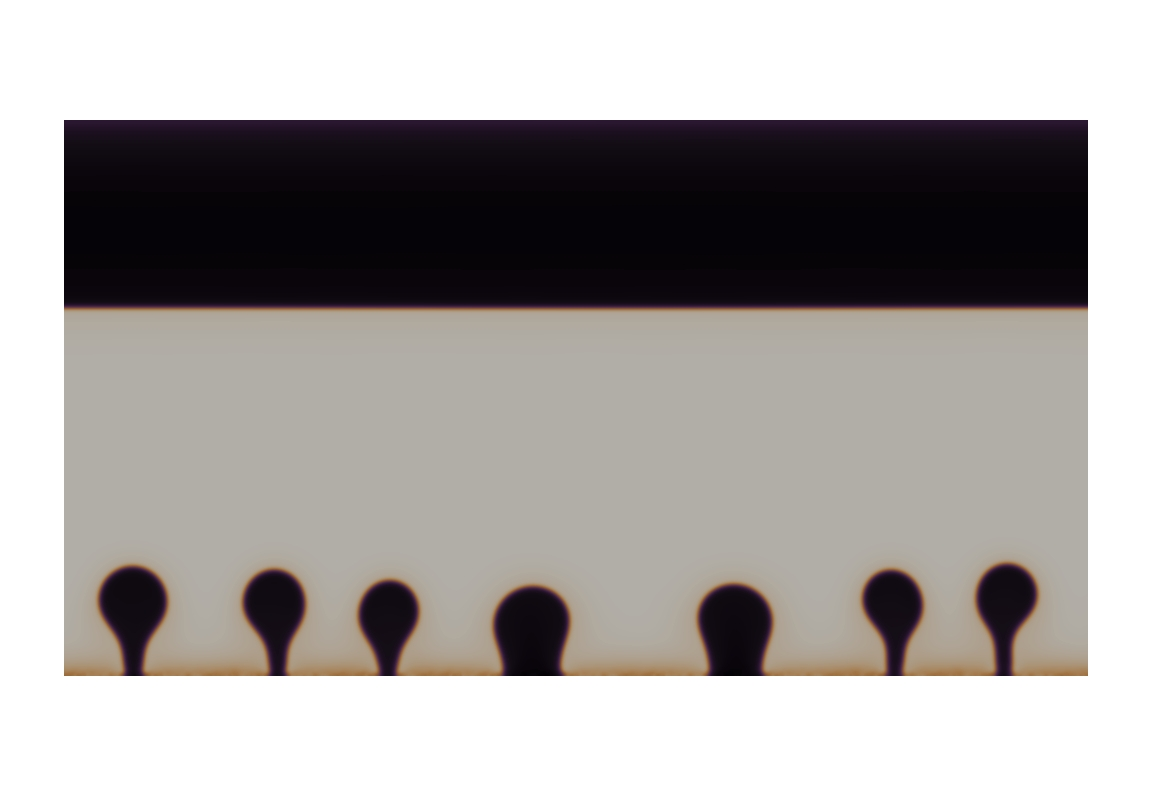
\includegraphics[width=0.8\textwidth]{Imagenes/HetBoiling/Placas6/t_34k}   
        \vspace{-10mm}
        \caption{$t^*=3.93$}     
    \end{subfigure}
    \begin{subfigure}[t]{0.9\textwidth}
        \centering
        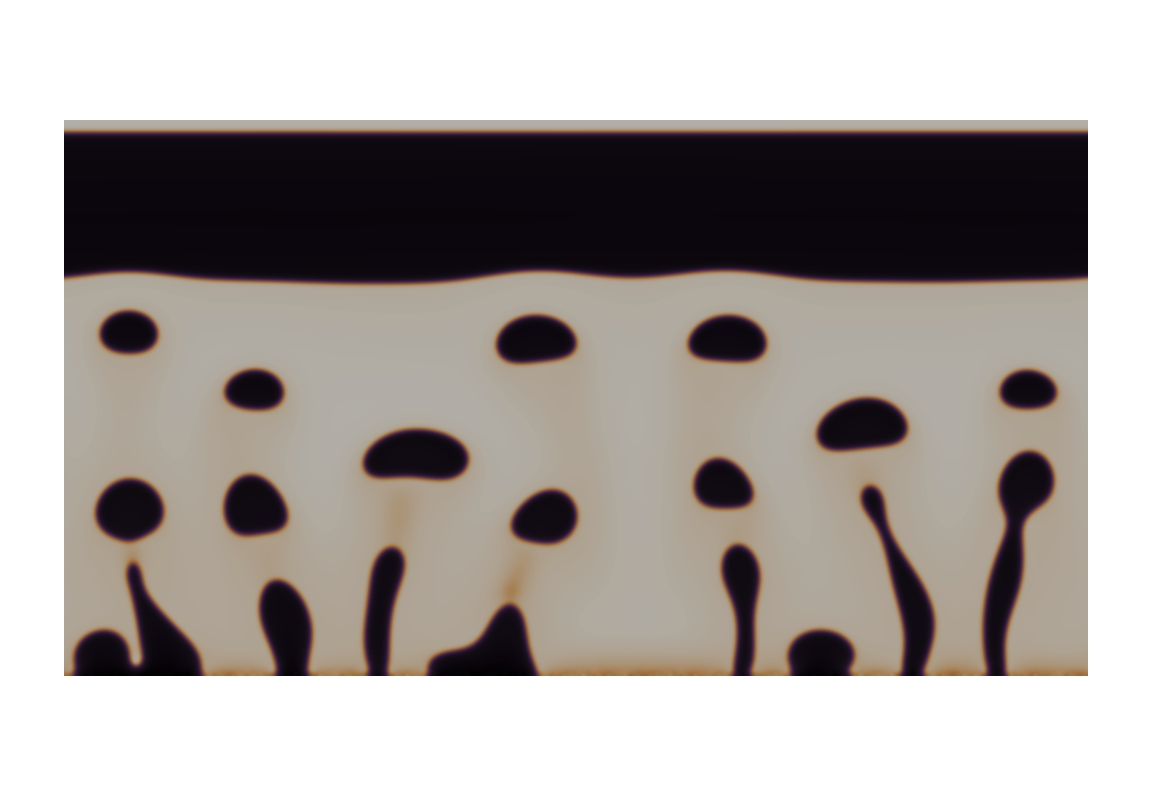
\includegraphics[width=0.8\textwidth]{Imagenes/HetBoiling/Placas6/t_80k}
        \vspace{-10mm}
        \caption{$t^*=9.24$}
    \end{subfigure}
    \begin{subfigure}[t]{0.9\textwidth}
        \centering
        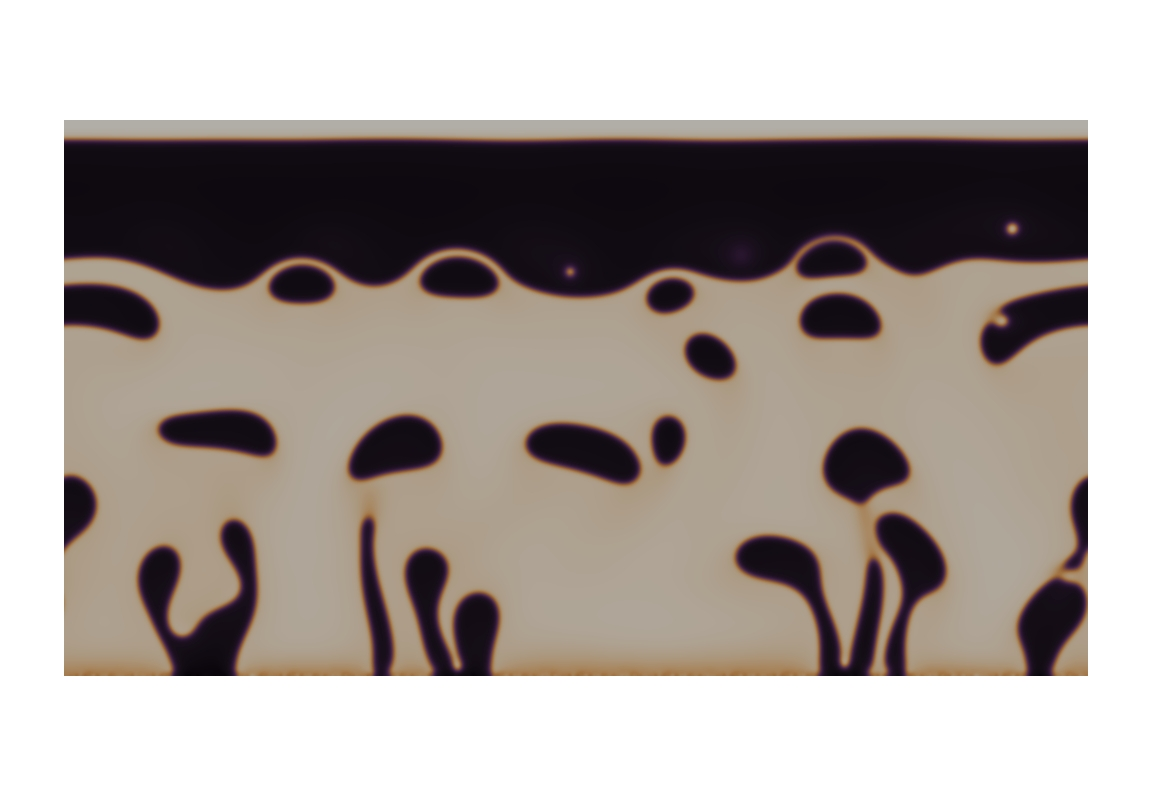
\includegraphics[width=0.8\textwidth]{Imagenes/HetBoiling/Placas6/t_120k}
        \vspace{-10mm}
        \caption{$t^*=13.86$}
    \end{subfigure}    
    \caption{Ebullici\'on sobre placas paralelas. $T_w=1.2\,T_c$.}
    \label{fig:nucleate}
\end{figure}



\begin{figure}[htb]
    \centering
    \begin{subfigure}[t]{0.9\textwidth}
        \centering
        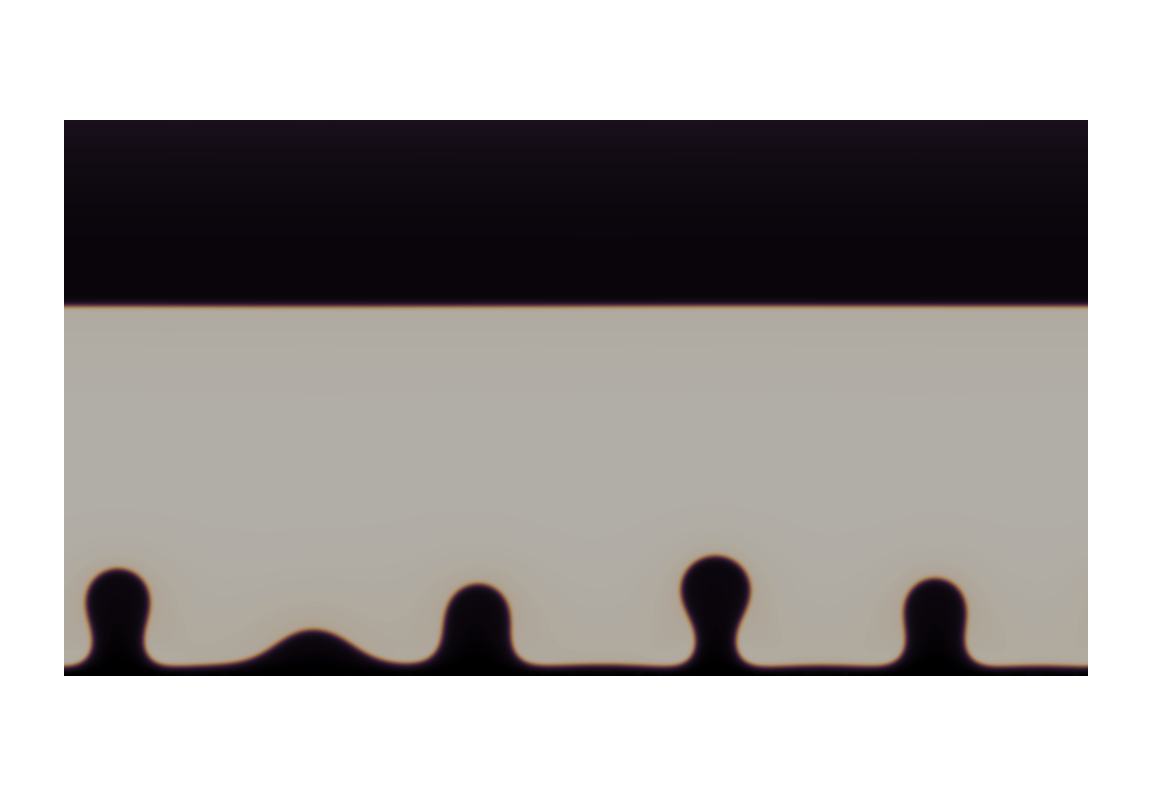
\includegraphics[width=0.8\textwidth]{Imagenes/HetBoiling/Placas7/t_140k}   
        \vspace{-10mm}
        \caption{$t^*=3.93$}     
    \end{subfigure}
    \begin{subfigure}[t]{0.9\textwidth}
        \centering
        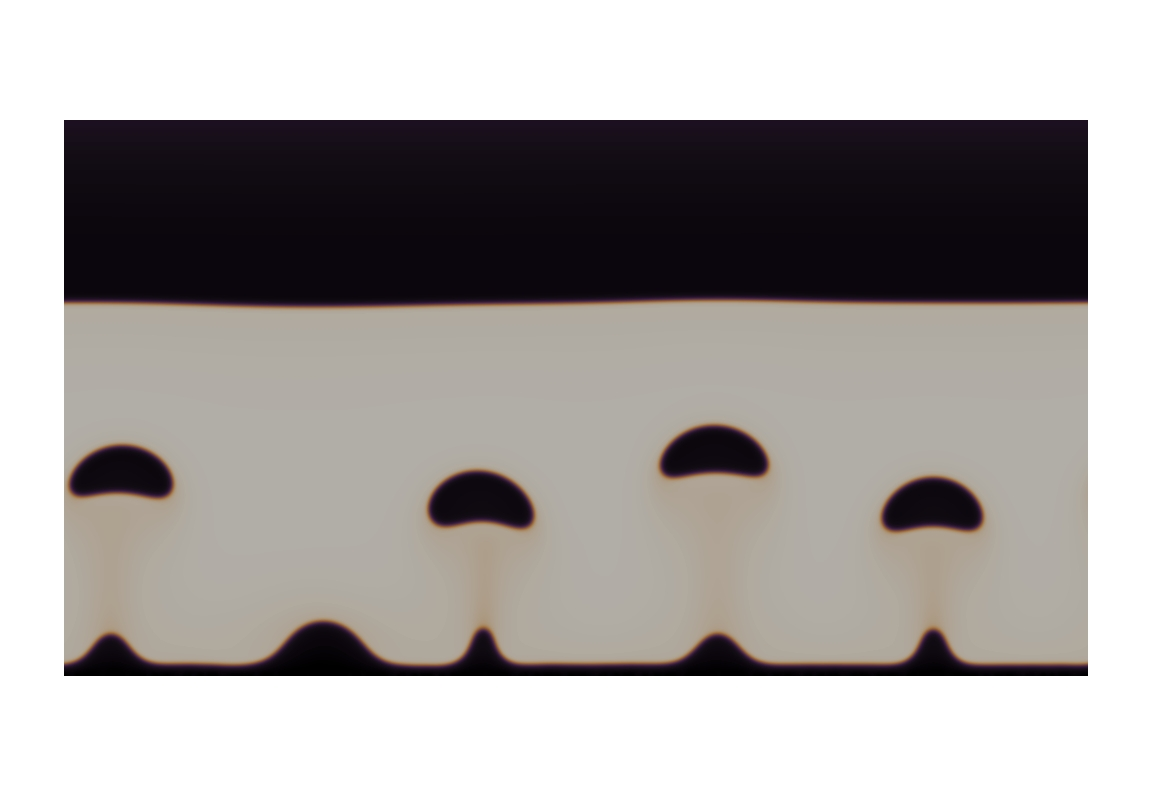
\includegraphics[width=0.8\textwidth]{Imagenes/HetBoiling/Placas7/t_160k}
        \vspace{-10mm}
        \caption{$t^*=9.24$}
    \end{subfigure}
    \begin{subfigure}[t]{0.9\textwidth}
        \centering
        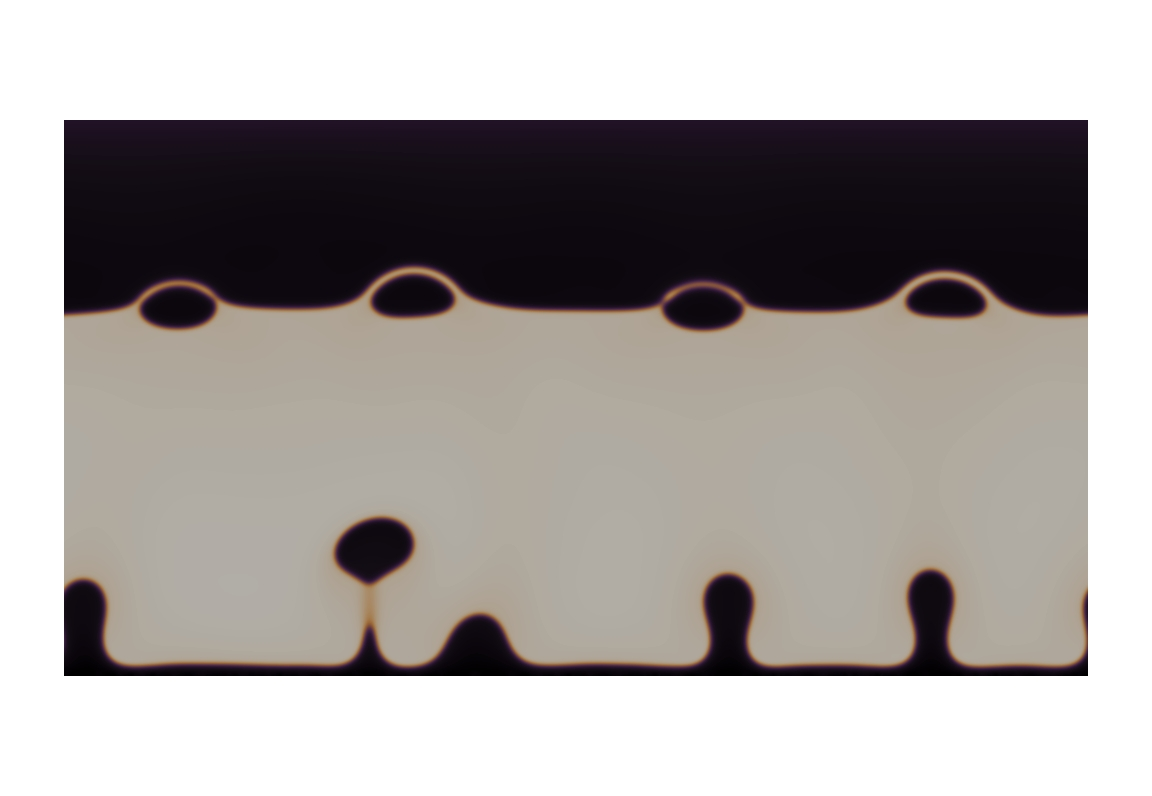
\includegraphics[width=0.8\textwidth]{Imagenes/HetBoiling/Placas7/t_200k}
        \vspace{-10mm}
        \caption{$t^*=13.86$}
    \end{subfigure}    
    \caption{Ebullici\'on sobre placas paralelas. $T_w=1.3\,T_c$.}
    \label{fig:film}
\end{figure}
\FloatBarrier




\section{Conclusiones}

En este cap\'itulo se introdujo un nuevo esquema de lattice Boltzmann en dos dimensiones, con dos funciones de distribuci\'on y operador de colisi\'on MRT, destinado a la resoluci\'on de flujos multif\'asicos con transferencia de calor. Este modelo acopla una \lbe{} de la familia \pp{} para resolver las ecuaciones hidrodin\'amicas, junto con una para el transporte de energ\'ia.

A diferencia de los esquemas de LB tradicionales, la estrategia propuesta introduce una adecuada definici\'on de la distribuci\'on de equilibrio directamente en el espacio de momentos, con par\'ametros libres que pueden usarse para ajustar la difusividad t\'ermica recuperada. Adem\'as, el an\'alisis de Chapman-Enskog muestra que cuando esta distribuci\'on de equilibrio se emplea junto con una matriz de relajaci\'on con coeficientes extra-diagonales no nulos, adecuadamente definidos, la ecuaci\'on de energ\'ia macrosc\'opica se recupera sin t\'erminos adicionales hasta la escala de expansi\'on analizada. De esta forma, no es necesario aplicar correcciones expl\'icitas a los t\'erminos de fuente o a la distribuci\'on post-colisi\'on, usualmente usadas para eliminar los efectos relacionados con la simulaci\'on de ecuaciones escalares de advecci\'on-difusi\'on usando esquemas LB cl\'asicos.

El modelo propuesto es capaz de reproducir problemas num\'ericos con soluciones anal\'iticas, como distribuci\'on de temperatura y densidad en un fluido vdW estratificado, as\'i como la evoluci\'on de la interfase en un problema de Stefan unidimensional. En el primer caso, el modelo es capaz de calcular adecuadamente las distribuciones en el centro del fluido y la posici\'on de la interfase para diferentes condiciones de contorno. De forma similar a lo observado en el caso isot\'ermico, se observa consistencia del m\'etodo en unidades reducidas. En la segunda prueba, la evoluci\'on de la posici\'on de la interfase pudo ser reproducida satisfactoriamente usando diferentes combinaciones de constantes de equilibrio y par\'ametros de relajaci\'on que conducen a una misma difusividad t\'ermica, lo que evidencia el cumplimiento del comportamiento previsto por la expansi\'on de Chapman-Enskog.

Por otro lado, se analiz\'o la consistencia y orden de convergencia del modelo propuesto mediante la simulaci\'on de generaci\'on de burbujas sobre una superficie horizontal calefaccionada. Para ello, se aplic\'o una evaluaci\'on de independencia de grilla de dos pasos, tomando como base la reproducci\'on de n\'umeros adimensionales caracter\'isticos. En primer lugar, se realizaron simulaciones sobre diferentes grillas, conservando estos par\'ametros junto con el espesor de interfase adimensional. En este caso, no se observaron diferencias significativas en la evoluci\'on de la interfase entre las distintas simulaciones, lo que constituye un claro indicio de que las ecuaciones macrosc\'opicas se recuperan seg\'un lo esperado. Adicionalmente, se realiz\'o un segundo conjunto de simulaciones sobre diferentes grillas, conservando los mismos n\'umeros adimensionales relevantes y el espesor de interfase en unidades de grilla. En este caso, el di\'ametro de partida adimensional converge con orden 2.18.

El problema de ebullici\'on heterog\'enea sirvi\'o adem\'as para verificar que la elecci\'on del m\'etodo para aplicar las condiciones de contorno influye significativamente en el proceso de crecimiento y desprendimiento de las burbujas. En particular, mientras que el modelo de Inamuro produce resultados consistentes con simulaciones efectuadas con una ecuaci\'on de energ\'ia resuelta por diferencias finitas, los m\'etodos de equilibrio y de extrapolaci\'on no conducen al rompimiento del cuello, y por lo tanto, evitan el desprendimiento de las burbujas. Una vez desarrollada la metodología para implementar la condici\'on de contorno y la grilla adecuada se determin\'o la dependencia del diámetro de partida con la gravedad y se verific\'o que sigue adecuadamente la ley propuesta en las correlaciones existentes.

Durante el desarrollo del modelo t\'ermico se propuso una alternativa para calcular el gradiente de temperatura expl\'icitamente en el t\'ermino de fuente, que s\'olo involucra a los valores locales de la funci\'on de distribuci\'on y de la distribuci\'on de equilibrio en cada nodo. Con este esquema, no se observaron diferencias significativas con los resultados obtenidos usando diferencias finitas centradas para $\nabla T$, lo que motiva al uso de este esquema en caso de requerir una optimizaci\'on de modelos de c\'alculo paralelizados.

Finalmente, simulaciones de ebullici\'on sobre placas planas, donde se considera una condici\'on de contorno de temperatura con fluctuaciones en torno a un valor medio, muestran que el modelo permite reproducir, a nivel cualitativo, fen\'omenos caracter\'isticos del proceso. Si bien estas simulaciones corresponden a dominios bidimensionales, y por lo tanto no a un caso real, se observ\'o que modificaciones en la temperatura de la superficie calefactora induce la generaci\'on de burbujas siguiendo patrones significativamente diferentes. En particular, en las condiciones de simulaci\'on presentadas se observ\'o una producci\'on de burbujas asociadas a diferentes reg\'imenes de ebullici\'on conocidos.
